\documentclass{article}
\usepackage[utf8]{inputenc} %кодировка
\usepackage[T2A]{fontenc}
\usepackage[english,russian]{babel} %русификатор 
\usepackage{mathtools} %библиотека матеши
\usepackage[left=1cm,right=1cm,top=2cm,bottom=2cm,bindingoffset=0cm]{geometry} %изменение отступов на листе
\usepackage{amsmath}
\usepackage{graphicx} %библиотека для графики и картинок
\graphicspath{}
\DeclareGraphicsExtensions{.pdf,.png,.jpg}
\usepackage{subcaption}
\usepackage{pgfplots}
\usepackage{float}
\usepackage{listings}


\lstset{
    numbers=left,            % Нумерация строк слева
    numberstyle=\tiny,       % Размер шрифта для номеров строк
    stepnumber=1,            % Нумеровать каждую строку
    numbersep=5pt,           % Расстояние между номерами и кодом
    backgroundcolor=\color{white},  % Цвет фона
    showspaces=false,        % Не показывать пробелы
    showstringspaces=false,  % Не показывать пробелы в строках
    showtabs=false,          % Не показывать табуляцию
    frame=single,            % Рамка вокруг кода
    tabsize=2,               % Размер табуляции
    breaklines=true,         % Автоматический перенос строк
    breakatwhitespace=true   % Переносить строки только по пробелам
}


\begin{document}
% НАЧАЛО ТИТУЛЬНОГО ЛИСТА
\begin{center}
    \Large
    Федеральное государственное автономное \\
    образовательное учреждение высшего образования \\ 
    «Научно-образовательная корпорация ИТМО»\\
    \vspace{0.5cm}
    \large
    Факультет программной инженерии и компьютерной техники \\
    Направление подготовки 09.03.04 Программная инженерия \\
    \vspace{1cm}
    \Large
    \textbf{Отчёт по лабораторной работе №1} \\
        По дисциплине «Распределённые системы хранения данных» ( семестр 6)\\
    \large
    \vspace{8cm}

    \begin{minipage}{.33\textwidth}
    \end{minipage}
    \hfill
    \begin{minipage}{.4\textwidth}
    
        \textbf{Студент}: \vspace{.1cm} \\
        \ Дениченко Александр P3312\\
        \textbf{Практик}:  \\
        \ Осипов Святослав
    \end{minipage}
    \vfill
Санкт-Петербург\\ 2025 г.
\end{center}
\pagestyle{empty}
% КОНЕЦ ТИТУЛЬНОГО ЛИСТА 
\newpage
\pagestyle{plain}

\section*{Задание}
Используя сведения из системных каталогов, получить информацию обо всех файлах данных, доступных для чтения и записи. Полученную информацию представить в следующем формате:

No. FILE\#	   CREATION\_TIME	   STATUS

 --- -----------   ----------------------  ------------------------------
  
 1 00000001      2014-09-10 00:00:00     ONLINE


\section*{Выполнение}

\begin{lstlisting}[caption={script.sql}, label={lst:example}]
CREATE OR REPLACE PROCEDURE show_files() LANGUAGE plpgsql AS $$
DECLARE
    X record;
BEGIN

    RAISE NOTICE 'No. FILE#      NAME      MODIFICATION_TIME           SPACE';
    RAISE NOTICE '--- ---------- -------   ---------------------       ------------';

    FOR X IN (
        select 
            ROW_NUMBER() OVER (ORDER BY(relfilenode)) as n, 
            relfilenode as node, 
            relname as rname, 
            (pg_stat_file(pg_relation_filepath(pg_class.oid))).modification as modif, 
            nspname as spac
        from pg_class 
        join pg_namespace on pg_namespace.oid = pg_class.relnamespace 
        where relkind = 'r' and nspname != 'pg_catalog' and nspname != 'information_schema'
    ) LOOP
        RAISE NOTICE '%    %    %    %    %',
            X.n::text,
            X.node::text,
            X.rname,
            to_char(X.modif::timestamp, 'YYYY-MM-DD HH24:MI:SS'),
            X.spac;
    END LOOP;
END;
$$;
\end{lstlisting}

\begin{lstlisting}[caption={kitty}, label={lst:example}]
postgres=# call show_files();
NOTICE:  No. FILE#      NAME      MODIFICATION_TIME           SPACE
NOTICE:  --- ---------- -------   ---------------------       ------------
NOTICE:  1    16389    users    2025-02-15 19:15:38    public
NOTICE:  2    16397    products    2025-02-15 19:15:38    public
NOTICE:  3    16455    u_order    2025-02-15 19:15:38    public
NOTICE:  4    16481    order_products    2025-02-15 19:15:38    public
NOTICE:  5    16497    data_directory    2025-02-19 10:16:39    public
CALL
\end{lstlisting}

\section*{Дополнительное задание}

Сделать систему хранения данных схожую с facebook на postgres и на MongoDB, провести анализ быстродействия и удобства.

\begin{center}
    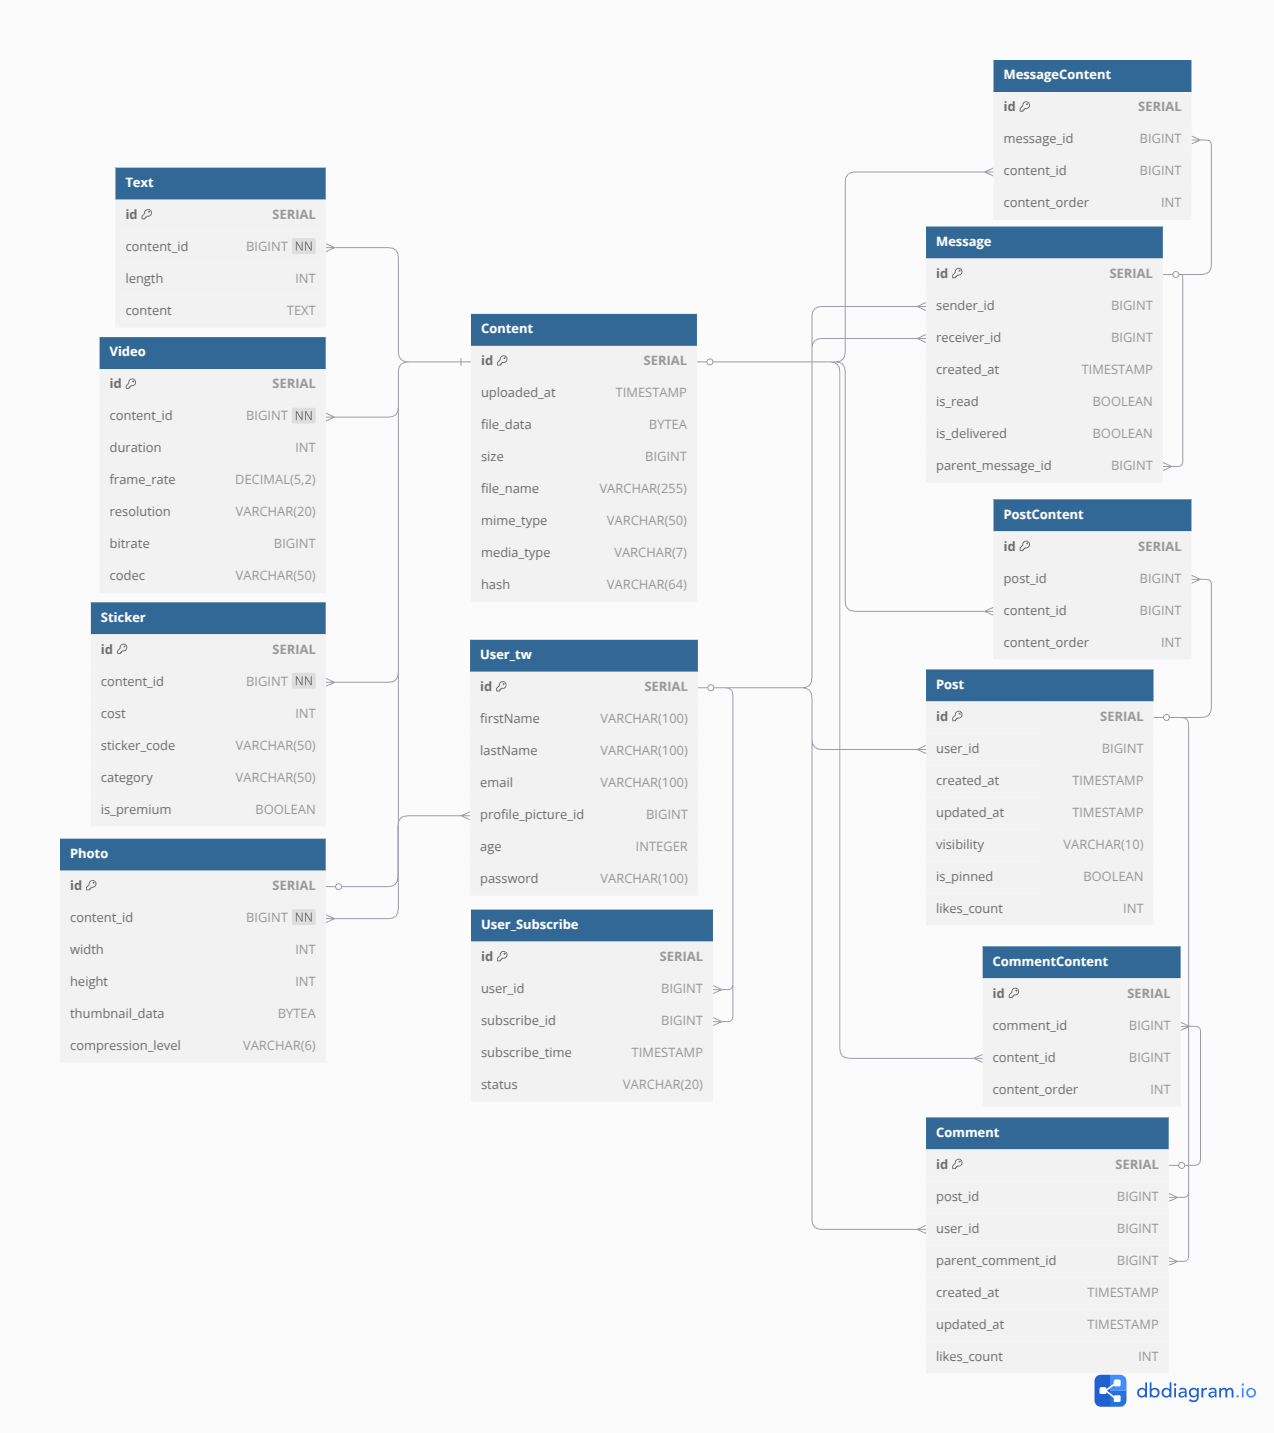
\includegraphics[width=1\textwidth]{postgres.png}
\end{center}

\end{document}
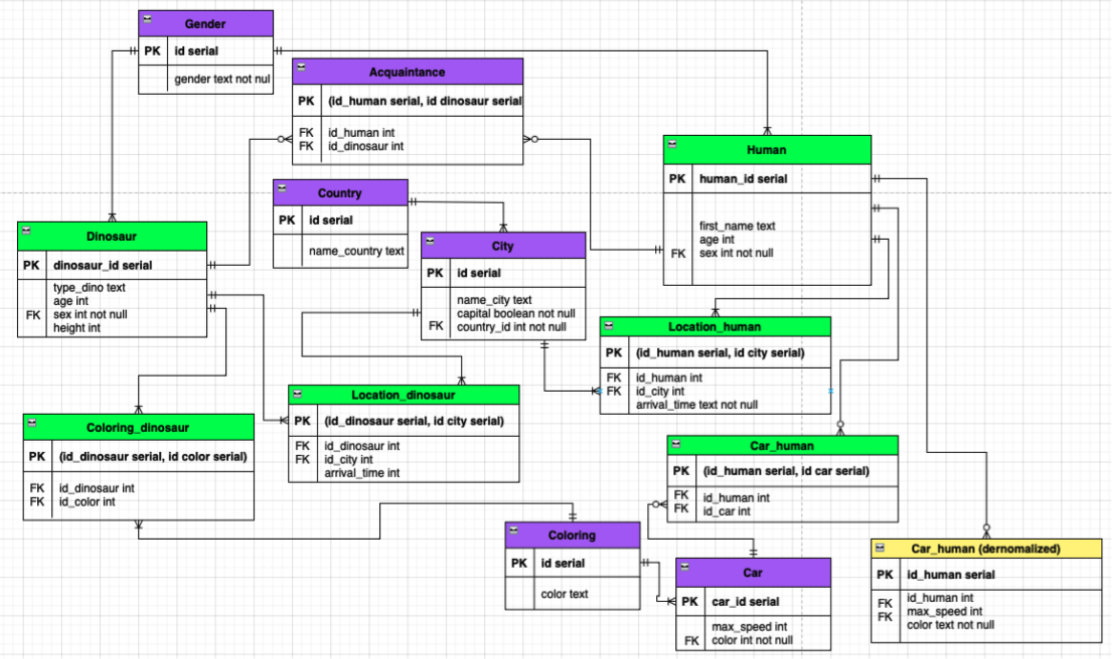
\includegraphics[width=.9\textwidth]{123}